\documentclass[a4paper,11pt,oneside]{article}
%Packages
\usepackage{amsmath}
\usepackage{graphicx}
\usepackage{fullpage}
\usepackage{graphicx}
\usepackage{tikz}
\definecolor{lichtgrijs}{gray}{0.95}
\setlength{\parskip}{\baselineskip}%vertical line spacing by new paragraph
\setlength{\parindent}{0cm}
\usepackage[english]{babel}
\usepackage{pgfplots}
\usepackage{gnuplot-lua-tikz}
\usepackage{epstopdf}
\epstopdfsetup{outdir=./}
\usepackage{algorithmic}
\usepackage{algorithm}
\usepackage{enumerate}
\usepackage{geometry}
\usepackage{caption}
\usepackage{chngpage}
\usepackage{tikz}
\usetikzlibrary{chains}
\usepackage{eurosym}
\def\arraystretch{1.5}
\usepackage{wrapfig}
\usepackage{enumitem}
\setlist[itemize]{noitemsep, topsep=2pt}
\setlist[enumerate]{noitemsep, topsep=2pt}
\usepackage{wrapfig}
\usepackage{subcaption}
\usepackage{import}
\usepackage[numbers]{natbib}
\usepackage{url}
\usepackage{tabularx}
\usepackage{listings}
%\usepackage[round]{natbib} % Voor auteur-jaar citaties
\usepackage[nottoc]{tocbibind} % Bibliografie in ToC; zie tocbibind.dvi
\usepackage[toc,page]{appendix}
\usepackage{xcolor}
\newcommand{\todo}[1]{\textbf{\textcolor{red}{TODO: #1}}\PackageWarning{TODO:}{TODO: #1!}}
\newlength{\Oldarrayrulewidth}
\newcommand{\Cline}[2]{%
  \noalign{\global\setlength{\Oldarrayrulewidth}{\arrayrulewidth}}%
  \noalign{\global\setlength{\arrayrulewidth}{#1}}\cline{#2}%
  \noalign{\global\setlength{\arrayrulewidth}{\Oldarrayrulewidth}}}
\bibliographystyle{bibliodutch}
\lstset{
	basicstyle=\scriptsize,
	backgroundcolor=\color{lichtgrijs},
	numbers=left,
	numberstyle=\tiny,
	numbersep=9pt,
	showspaces=false,
	showstringspaces=false,
	showtabs=false,
	frame=leftline,
	tabsize=2,
	captionpos=b,
	title=\lstname,
	breaklines=true,
	breakatwhitespace=true,
	stepnumber=4
}
\lstdefinestyle{customc}{
  belowcaptionskip=1\baselineskip,
  breaklines=true,
  language=R,
  showstringspaces=false,
  basicstyle=\footnotesize\ttfamily,
  keywordstyle=\bfseries\color{green!40!black},
  commentstyle=\itshape\color{purple!40!black},
  stringstyle=\color{orange},
}

\begin{document}

%  Titelblad

% Opmerking: gaat uit van een \baselinestretch waarde van 1.5 (die moet
% ingesteld worden voor het begin van de document environment)

\begin{titlepage}
\pagenumbering{gobble}% Remove page numbers (and reset to 1)
\clearpage
\newgeometry{top=2cm, bottom=2cm, right=1.5cm, left=1.5cm}

%logo
\begin{figure}[!ht]
  \begin{adjustwidth}{-1.5cm}{}
    \centering
    
\includegraphics[width=\paperwidth]{logo.jpg}
  \end{adjustwidth}
\end{figure}

\begin{center}

\fontsize{12pt}{14pt}
\selectfont
 
\vspace{6cm} 
\Huge \textsc{Design of Multimedia Applications:}\\ 
\vspace{1cm}
\huge
\textsc{Video Shot Detection, Annotation,\\ and Retrieval}\\
\vspace{10.5cm}
\Large
Group 40:\\
Eveline Hoogstoel, Titouan Vervack and Dries Wijns\\
$1^{st}$ Master in Computer Science Engineering


\end{center}
\end{titlepage}

\thispagestyle{empty}

\pagebreak

\newgeometry{left=2.5cm,right=2.5cm,bottom=2.5cm, top=2.5cm}
\pagenumbering{arabic}% Arabic page numbers (and reset to 1)

\section{Implementation of method 5}
The shot detection used in exercise 5 works by calculating the structural similarity (SSIM) index (equation \ref{ssim}) between two adjacent frames. The structural similarity is calculated on a sliding window, and the final index is the mean SSIM over all the windows.
If this final index falls below a threshold, we say that a shot has occurred. An important thing to note is that the SSIM is calculated on the luma component of the images, an does not use any chrominance information.

\begin{equation}
\label{ssim}
 \Delta E = \frac{\sigma_{xy}}{\sigma_x \sigma_y} \frac{2 \mu_x \mu_y}{\mu_x^2 + \mu_y^2} \frac{2 \sigma_x \sigma_y }{\sigma_x^2 + \sigma_y^2}
\end{equation}



\begin{lstlisting}
let z be the sliding-window with (in pixels)
let w be the frame width (in pixels)
let h be the frame height (in pixels)

total_ssim = 0
nr_comparisons = 0

for x from 0 to w-z do:
	for y from 0 to h-z do:
    	mu_x = mean luma in window over current frame
        mu_y = mean luma in window over previous frame
        sigma_x = luma variance in window over current frame
        sigma_y = luma variance in window over previous frame
        sigma_xy = luma crossvariation in window between current frame an previous frame
        
        //c_1 and c_2 are fixed values to make the devision more stable
        c_1 = 0.01
        c_2 = 0.03
        
        ssim = ((2*mu_x*mu_y+c1)(2*sigma_xy+c_2))/((mu_x^2+mu_y^2+c1)(sigma_x^2+sigma_y^2+c2))
        total_ssim += ssim
        nr_comparisons += 1

mean_ssim = total_ssim/nr_comparisons

if mean_ssim < threshold:
	return True  // yes, a cut has been detected
return False  // no cut has been detected
\end{lstlisting}
\vspace{-1cm}
\section{Used parameters and explanatory notes}
\vspace{-0.5cm}
In our software we handed in the most thresholds had no maximum value, for the test we have normalized the results of each algorithm so we have an upper bound for these thresholds. \\
The meaningful subset for blocksizes or regionsizes is always 8 - 64 since these sizes are not too big yet contain enough information. The meaningful subsets for complete window sizes (left to right boundary of window) are always 8 - 128 this is related to the block- and regionsizes, we always want at least two block in the search window and usually even a few more.\\
For SSIM: the ssim index will lie within -1 to 1. A ssim index of 1 means the two frames are identical. A good threshold value lies within 0 to 0.2, meaning some motion is allowed within a shot, but a complete change of scene will be detected. The sliding window size can be from 1 by 1 pixels to the whole frame. A good value would be 8 by 8 pixels, which is a clearly visible block with structural information.\\
\begin{tabularx}{\textwidth}{|l|X|c|c|}
\cline{1-4}
\multicolumn{1}{|c|}{\textbf{Parameters}}&\multicolumn{1}{|c|}{\textbf{Definition}}&\textbf{Range}&\textbf{Meaningful subset}\\
\Cline{3pt}{1-4}
\multicolumn{4}{|c|}{\textbf{Pixel Difference}}\\
\Cline{2pt}{1-4}
Threshold 1&Threshold for the allowed difference between two pixels&0 - 765&100 - 200\\
\cline{1-4}
Threshold 2&Threshold to evaluate the frame difference computed by Pixel Difference&0 - $\infty$&30 - 100\\
\Cline{2pt}{1-4}
\multicolumn{4}{|c|}{\textbf{Motion Estimation}}\\
\Cline{2pt}{1-4}
Threshold&Used to determine how well the sum of all blocks between two frames compare to each other&0 - 10& 1-5\\
\cline{1-4}
Block size&Size of blocks in which the frame is divided&0 - frameResolution&8 - 64\\
\cline{1-4}
Search window size&Distance in pixels of the center block of the search window to its boundary&0 - $\frac{frameResolution}{2}$&8 - 128\\
\Cline{2pt}{1-4}
\multicolumn{4}{|c|}{\textbf{Global Histogram}}\\
\Cline{2pt}{1-4}
Threshold&Threshold to evaluate the frame difference computed by Global Histogram&0 - 100& 0-30\\
\cline{1-4}
Number of bins&Amount of bins to use&1 - 765&8 - 16\\
\Cline{2pt}{1-4}
\multicolumn{4}{|c|}{\textbf{Local Histogram}}\\
\Cline{2pt}{1-4}
Threshold&Threshold to evaluate the frame difference computed by Local Histogram&0 - 100&0-30\\
\cline{1-4}
Number of bins&Amount of bins to use&1 - 765&8 - 16\\
\cline{1-4}
Region size&Size of a region, frame will be cut into regions&0 - frameResolution&8 - 64\\
\Cline{2pt}{1-4}
\multicolumn{4}{|c|}{\textbf{Structural Similarity Index}}\\
\Cline{2pt}{1-4}
Threshold&If the structural similarity index of the two frames falls below this threshold, a cut has been detected&(-1) - 1&0 - 0.2\\
\cline{1-4}
Region size&The total width (in pixels) for the sliding window&0 - frameResolution&8 - 64\\
\cline{1-4}
\end{tabularx}\par

\vspace{-0.5cm}
\section{Precision and recall}
\vspace{-0.5cm}
When looking at all the results; we notice a similar trend. If we want more recall, we lose
precision. This means that we find more shots, but we also find more false shots.
\vspace{-0.5cm}
\section{Computational complexity}
\vspace{-0.5cm}
\textit{Note: The local histogram that was handed in still contained errors which we fixed in to be able to get correct result. The handed in version looped over the blocks (there were always 9 blocks) and then looped over the regionSize twice. The corrected version first divides the frames into squares of regionSizeXregionSize and then loops over these blocks and calculates their histograms.}\par
The execution time of Pixel Difference is independent of its parameters. It only depends on the resolution of the video as it just loops over both loops pixelwise.\par
The execution time of Motion Estimation is mostly dependent on its parameters (not on threshold). Motion Estimation iterates of all of the blocks in the current frame and then iterates over a search window in the next frame. Because of constant searching over a search window it will be slower in comparison to Pixel Difference. Varying the search window size will have the biggest impact on the performance of the algorithm.\par
Global histogram is another very easy algorithm, just like Pixel Difference it just loops over both of the frames pixelwise. Making changes to the parameters should hardly impact the execution time of the algorithm. The only parameter that has an impact on the performance is the \textit{amount of bins}. This is because at the end of the algorithm the distance between the two frames still has to be calculated. For this we have to loop once over the amount of bins. The algorithm should have roughly the same execution time as Pixel Difference (a little longer because of the distance calculation).\par
Local Histogram's computation time shouldn't be too different from Global Histogram. Local Histogram first divides the frames into blocks and then goes over each block pixelwise. This has the same complexity as Global Histogram, the only difference is in the calculation of the distance between two frames. For this calculation we now have to loop over the amount of block and the amount of bins. This means that both the amount of bins and the regionSize will have an impact on the execution speed of Local Histogram\par
For the Stuctural Similarity Index, the number of pixel values read is in function of the window size.
\begin{equation}
N = (w-z)(h-z)(z^2) = O(z^4)
\end{equation}\par
Where $w$ is the width of the frame in pixel, $h$ the height and $z$ the regionSize.
\vspace{-0.5cm}
\subsection{Time measurements}
\vspace{-0.5cm}
For all measurements we have used the following hardware and software:
\begin{itemize}
	\item \textbf{CPU:} Intel I7-4790S quad core @4.0Ghz
	\item \textbf{RAM:} 8GB @1600Mhz
	\item \textbf{SSD:} Samsung 840 evo 250GB, 540MB/s sequential read, 97.000 IOPS (4K random reads)
	\item \textbf{OS:} Windows 8.1 64-bit\\
\end{itemize}
The local histogram algorithm has a linear complexity. You can see this in figure \ref{fig:time_LH}, where the time measurements of the \verb!csi.avi! file are plotted.
\begin{figure}[H]
\centering
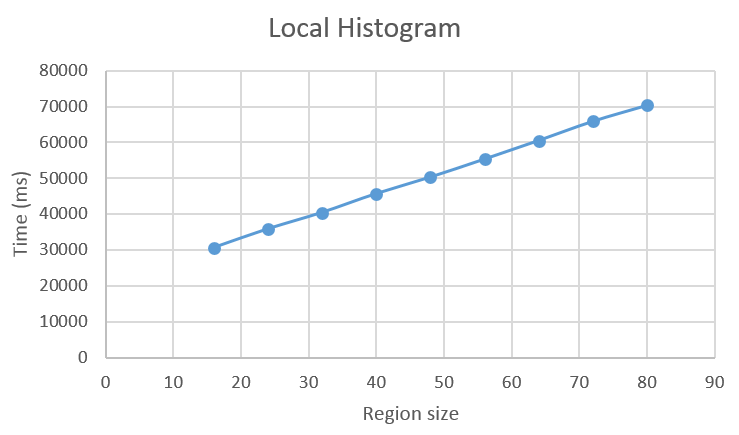
\includegraphics[width=0.6\textwidth]{img/time_LH.png}
\caption{Time measurements of local histogram algorithm}\label{fig:time_LH}
\end{figure}
The motion estimation algorithm is dependent on 2 parameters: \verb!blocksize! and \verb!searchwindow size!. In figure \ref{subfig:1} we can see that the time is quadratic dependent on the \verb!searchwindow size!. And in \ref{subfig:2} you can see that the computation time decreases enormous if the blocksize increases.
\begin{figure}[H]
        \begin{subfigure}[h]{0.5\textwidth}
                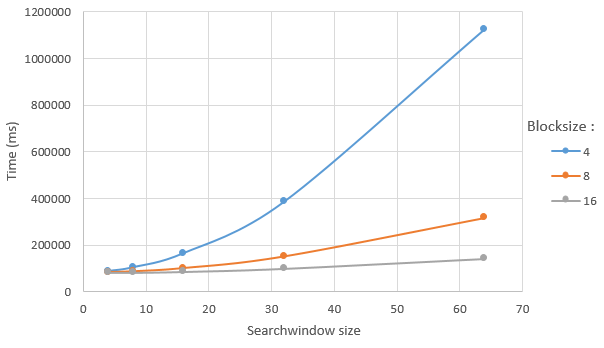
\includegraphics[width=\textwidth]{img/time_motion_1.png}
                \caption{ }\label{subfig:1}
        \end{subfigure}%
        ~
        \begin{subfigure}[h]{0.5\textwidth}
                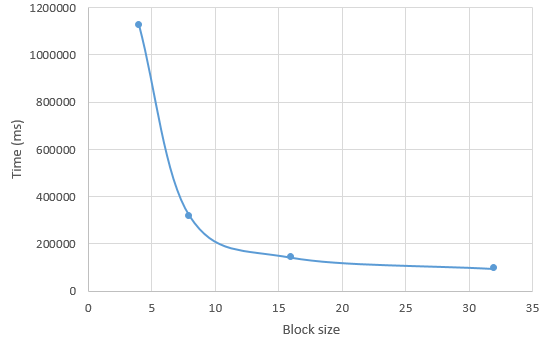
\includegraphics[width=\textwidth]{img/time_motion_2.png}
                \caption{ }\label{subfig:2}
        \end{subfigure}
        \caption{Time measurements for motion estimation}\label{fig:time_motion}
\end{figure}
The other algorithm execute in a constant time. You can see the time measurements in table \ref{tab:times} for the \verb!return_jedi_trailer_cuts-only.avi! file.
\begin{table}[H]
\centering
\begin{tabular}{l|r}
Algorithm & Time (ms)\\
\hline
Global histogram & $\pm$ 81000\\
Pixel difference & $\pm$ 75000\\
\end{tabular}
\caption{Time measurements}
\label{tab:times}
\end{table}
And for method 5 we have no time measurements.
\section{ROC curves}
In figure \ref{fig:ROC} you can see the ROC curve for the \verb!return_jedi_trailer_cuts-only.avi! file. We were not able to process other video fragments in time.
\begin{figure}[H]
\centering
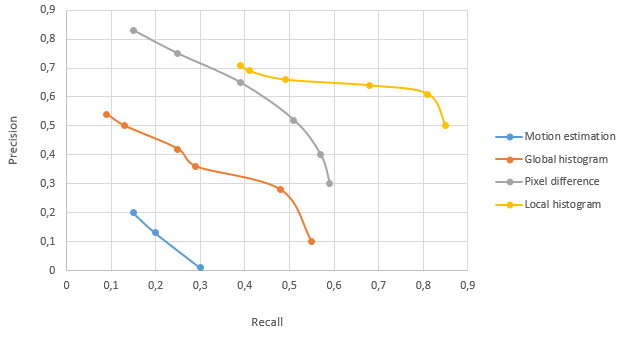
\includegraphics[width=0.8\textwidth]{img/ROC_jedi.png}
\caption{ROC-curve}\label{fig:ROC}
\end{figure}

\section{Comparison of the recall and precision against computational complexity}
According to the ROC curves motion estimation is the worst out of our algorithms. Followed by global histogram and local, pixel difference and local histogram. This means that local histogram is our best algorithm for precision and recall. Motion estimation would need more movement and a big search window to be able to produce good results. Pixel difference just checks the difference in pixel values, but since cuts usually have a different environment, the pixel values change drastically resulting in quite decent results. As global histogram is just a generalisation of local histogram it will always perform worse than local. Local histogram performs the best since it can be seen as a specialised version of pixel difference and global histogram, it checks for color differences on a frame level. In comparison to global histogram it is better because it can also detect changes where the distribution of pixel values doesn't change much. SSIM is based purely on the luma component which means that if two adjacent frames have roughly the same luma but completely different chrominance values, the cut won't be detected. This will negatively impact the precision of the algorithm.\\
If we compare the execution times we find that structural similarity index is our slowest algorithm, this is followed by motion estimation, local histogram, global histogram and finally pixel difference. The reason for the difference in execution time has been explained before in exercise 4.
\section{Questions}
\textbf{Question 1:}\\
According to the ROC curves local histogram is the clear winner, it is a bit slower than pixel difference and global histogram but it has the same complexity meaning it is a also a very good choice computation wise.\\
\textbf{Question 2:}\\
If a scene (very) slowly fades out this might not be detected by local histogram as the difference in color isn't big enough. A technique to detect this fading would increase the algorithms precision.\\
\textbf{Question 3:}\\
Local histogram does it work on blocks and each block is independent of the other, this means we could use multiple threads to speed up this process. A GPU would be fit a lot better for this task than a CPU since its strength lies in doing a lot of the same calculations at the same time. We can conclude that panellization is a good way to decrease the computation speed.
\textbf{Question 4:}\\
One obvious shortcoming is that all the algorithms are slow. Using these algorithm today, on high definition, 60fps video files, would be impractical. One way to deal with this is to reduce the information present in the video. For example: scale down the video to 720 by 480 pixels per frame, and reduce to only 4 or 12 frames per second.\\
\textbf{Question 5:}\\
In a normal video scene the camera is, compared to the background and the subject, relatively static. When filming with a wearable device, there will be a lot more movement from the camera. In order to overcome this problem, some strong and reliable video stabilization must be done before doing the shotdetection. \\
\textbf{Question 6:}\\
Now a days there is many video content on the web or even on our own pc, smartphone,... But sometime you are looking for a certain shot or a part of video. You can perfectly imagine how it looks but it's hard to find the right video because you do not know of which video it is a part. In that case it would be very useful if you can just press \verb!ctrl F! en look for some keywords. So in the case you have a huge amount of video files it is important to add metadata so you easily can search through the content.\\
\textbf{Question 7:}\\
The first problem we can foresee is that the way of annotating is completely free to the user. The user can choose the language or how to explain something. This means that there is no structure in the annotations. Because of this it can happen that a user is searching for a certain parameter and the program doesn't find all of the related shots. To solve this problem we could make use of an ontology such as OWL to give a structure to the annotation and to resolve ambiguity.
\end{document}
